\section{mo\-No\-Fit\-Impr\-Sol\-Continue$<$ EOT $>$ Class Template Reference}
\label{classmo_no_fit_impr_sol_continue}\index{moNoFitImprSolContinue@{moNoFitImprSolContinue}}
One possible stop criterion for a solution-based heuristic.  


{\tt \#include $<$mo\-No\-Fit\-Impr\-Sol\-Continue.h$>$}

Inheritance diagram for mo\-No\-Fit\-Impr\-Sol\-Continue$<$ EOT $>$::\begin{figure}[H]
\begin{center}
\leavevmode
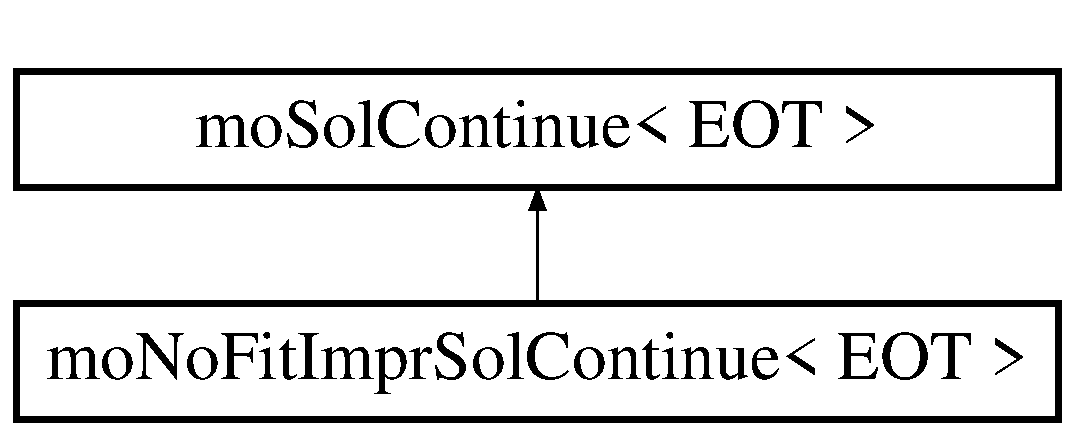
\includegraphics[height=4cm]{classmo_no_fit_impr_sol_continue}
\end{center}
\end{figure}
\subsection*{Public Types}
\begin{CompactItemize}
\item 
typedef EOT::Fitness {\bf Fitness}\label{classmo_no_fit_impr_sol_continue_w0}

\begin{CompactList}\small\item\em Alias for the fitness. \item\end{CompactList}\end{CompactItemize}
\subsection*{Public Member Functions}
\begin{CompactItemize}
\item 
{\bf mo\-No\-Fit\-Impr\-Sol\-Continue} (unsigned int \_\-max\-Number\-Of\-Iteration\-Without\-Improvement)
\begin{CompactList}\small\item\em Basic constructor. \item\end{CompactList}\item 
bool {\bf operator()} (const EOT \&\_\-solution)
\begin{CompactList}\small\item\em Function that activates the stopping criterion. \item\end{CompactList}\item 
void {\bf init} ()
\begin{CompactList}\small\item\em Procedure which allows to initialise all the stuff needed. \item\end{CompactList}\end{CompactItemize}
\subsection*{Private Attributes}
\begin{CompactItemize}
\item 
unsigned int {\bf max\-Number\-Of\-Iterations\-Without\-Improvement}\label{classmo_no_fit_impr_sol_continue_r0}

\begin{CompactList}\small\item\em Maximum number of iterations without improvement allowed. \item\end{CompactList}\item 
bool {\bf first\-Fitness\-Saved}\label{classmo_no_fit_impr_sol_continue_r1}

\begin{CompactList}\small\item\em Flag that this is the first time that the fitness is used. \item\end{CompactList}\item 
{\bf Fitness} {\bf fitness}\label{classmo_no_fit_impr_sol_continue_r2}

\begin{CompactList}\small\item\em Current Fitness. \item\end{CompactList}\item 
unsigned int {\bf counter}\label{classmo_no_fit_impr_sol_continue_r3}

\begin{CompactList}\small\item\em The iteration couter. \item\end{CompactList}\end{CompactItemize}


\subsection{Detailed Description}
\subsubsection*{template$<$class EOT$>$ class mo\-No\-Fit\-Impr\-Sol\-Continue$<$ EOT $>$}

One possible stop criterion for a solution-based heuristic. 

The stop criterion corresponds to a maximum number of iterations without improvement. 



Definition at line 46 of file mo\-No\-Fit\-Impr\-Sol\-Continue.h.

\subsection{Constructor \& Destructor Documentation}
\index{moNoFitImprSolContinue@{mo\-No\-Fit\-Impr\-Sol\-Continue}!moNoFitImprSolContinue@{moNoFitImprSolContinue}}
\index{moNoFitImprSolContinue@{moNoFitImprSolContinue}!moNoFitImprSolContinue@{mo\-No\-Fit\-Impr\-Sol\-Continue}}
\subsubsection{\setlength{\rightskip}{0pt plus 5cm}template$<$class EOT$>$ {\bf mo\-No\-Fit\-Impr\-Sol\-Continue}$<$ EOT $>$::{\bf mo\-No\-Fit\-Impr\-Sol\-Continue} (unsigned int {\em \_\-max\-Number\-Of\-Iteration\-Without\-Improvement})\hspace{0.3cm}{\tt  [inline]}}\label{classmo_no_fit_impr_sol_continue_a0}


Basic constructor. 

\begin{Desc}
\item[Parameters:]
\begin{description}
\item[{\em \_\-max\-Number\-Of\-Iteration\-Without\-Improvement}]The number of iterations without fitness improvement to reach for stop. \end{description}
\end{Desc}


Definition at line 57 of file mo\-No\-Fit\-Impr\-Sol\-Continue.h.

References mo\-No\-Fit\-Impr\-Sol\-Continue$<$ EOT $>$::counter, mo\-No\-Fit\-Impr\-Sol\-Continue$<$ EOT $>$::first\-Fitness\-Saved, and mo\-No\-Fit\-Impr\-Sol\-Continue$<$ EOT $>$::max\-Number\-Of\-Iterations\-Without\-Improvement.

\subsection{Member Function Documentation}
\index{moNoFitImprSolContinue@{mo\-No\-Fit\-Impr\-Sol\-Continue}!operator()@{operator()}}
\index{operator()@{operator()}!moNoFitImprSolContinue@{mo\-No\-Fit\-Impr\-Sol\-Continue}}
\subsubsection{\setlength{\rightskip}{0pt plus 5cm}template$<$class EOT$>$ bool {\bf mo\-No\-Fit\-Impr\-Sol\-Continue}$<$ EOT $>$::operator() (const EOT \& {\em \_\-solution})\hspace{0.3cm}{\tt  [inline, virtual]}}\label{classmo_no_fit_impr_sol_continue_a1}


Function that activates the stopping criterion. 

Indicates if the fitness has not been improved since a given number of iterations (after a minimum of iterations). \begin{Desc}
\item[Parameters:]
\begin{description}
\item[{\em \_\-solution}]the current solution. \end{description}
\end{Desc}
\begin{Desc}
\item[Returns:]true or false. \end{Desc}


Implements {\bf eo\-UF$<$ const EOT \&, bool $>$}.

Definition at line 67 of file mo\-No\-Fit\-Impr\-Sol\-Continue.h.

References mo\-No\-Fit\-Impr\-Sol\-Continue$<$ EOT $>$::counter, mo\-No\-Fit\-Impr\-Sol\-Continue$<$ EOT $>$::first\-Fitness\-Saved, and mo\-No\-Fit\-Impr\-Sol\-Continue$<$ EOT $>$::fitness.\index{moNoFitImprSolContinue@{mo\-No\-Fit\-Impr\-Sol\-Continue}!init@{init}}
\index{init@{init}!moNoFitImprSolContinue@{mo\-No\-Fit\-Impr\-Sol\-Continue}}
\subsubsection{\setlength{\rightskip}{0pt plus 5cm}template$<$class EOT$>$ void {\bf mo\-No\-Fit\-Impr\-Sol\-Continue}$<$ EOT $>$::init ()\hspace{0.3cm}{\tt  [inline, virtual]}}\label{classmo_no_fit_impr_sol_continue_a2}


Procedure which allows to initialise all the stuff needed. 

It can be also used to reinitialize all the needed things. 

Implements {\bf mo\-Sol\-Continue$<$ EOT $>$} {\rm (p.\,\pageref{classmo_sol_continue_a0})}.

Definition at line 102 of file mo\-No\-Fit\-Impr\-Sol\-Continue.h.

References mo\-No\-Fit\-Impr\-Sol\-Continue$<$ EOT $>$::counter, and mo\-No\-Fit\-Impr\-Sol\-Continue$<$ EOT $>$::first\-Fitness\-Saved.

The documentation for this class was generated from the following file:\begin{CompactItemize}
\item 
mo\-No\-Fit\-Impr\-Sol\-Continue.h\end{CompactItemize}
